\documentclass[12pt]{article}
\usepackage[dutch]{babel}

\usepackage{amsmath}
\usepackage{graphicx} 
\usepackage{lscape}



\author{Joshua de Bie - s1442627\\Thomas Raaijen - s1462431\\Josje van 't Padje - s1423037\\Gerwin Puttenstein - s1487779}
\date{\today}
\title{Integrated Project Netwerk Systemen\footnote{Made in \LaTeX} \\ Let us begin talkin'!}

\begin{document}
\maketitle
\thispagestyle{empty}
\setcounter{page}{0}
\newpage

\tableofcontents
\newpage

\section{Introductie}
In dit artikel wordt het integrated project besproken.\\ Met het integrated project is het de bedoeling om een chatapplicatie te ontwerpen dat het Ad hoc netwerk setup implementeert. Het onderwerp chatapplicaties is interessant, omdat in de afgelopen tijd Whatsapp vaak in het nieuws kwam na de overname door Facebook. Whatsapp zou veel gebruikers hebben verloren aan een andere chatapplicatie genaamd "Telegram". Whatsapp verloor zoveel gebruikers, omdat deze gebruikers bang waren om hun privacy te verliezen. Daarom is het van belang dat er een chatapplicatie komt die gebruik maakt van (as)symmetrische sleutels, om de privacy van zijn gebruikers te waarborgen. In dit artikel word de gemaakte chatapplicatie gepresenteerd die extensief gebruik zal maken van de bekende beveiligingsmethoden.\\
Dit artikel wordt opgebouwd met het welbekende IMRAD-structuur, dit wil zeggen dat eerste de ge\"implementeerde ontwerp keuzes en methoden aan bod komen en daarna de de resultaten worden gepresenteerd en daaraan een korte conclusie gegeven wordt. Wij zullen ons eerst kort introduceren aan de hand van onze functie binnen het project. Vervolgens zal het ontwerp van onze chatapplicatie aanbod komen met onze keuzes als het gaat om het interne netwerk systeem, daarna zal er over gegaan worden naar het grafische ontwerp aanbod komen. De resultaten van beiden ontwerpen zullen besproken en zal er een korte conclusie getrokken worden. 
\newpage

\section{Functies binnen het team}
\label{taken}
\textbf{Gerwin} \\
\emph{Lead Designer Network Systems} \\
Gerwin zorgt ervoor dat het netwerk gedeelte van het project structuur krijgt en dat de rest van het team hiermee aan de slag kan zonder alles uit te moeten zoeken.
\\

\noindent\textbf{Joshua} \\
\emph{Lead Designer Software Systems} \\
Joshua zorgt ervoor dat het software gedeelte van het project goed gestructureerd wordt. Dit wil zeggen dat de klassen van het project overzichtelijk en voorzien worden van het nodige commentaar.
\\

\noindent\textbf{Josje} \\
\emph{Spokeswoman} \\
Josje is het vliegende teamlid, zij gaat iedereen ondersteunen waar nodig is en houd een oogje in het zeil. 
\\

\noindent\textbf{Thomas} \\
\emph{Chairman} \\
Thomas zorgt voor alle verslagen en dat iedereen zijn of haar taak uitvoert. Zelf zou hij overal bijvallen en de besprekingen leiden. Ook moet hij ervoor zorgen dat er een koers wordt gevaren. Ook zal hij de overzicht in de drive moeten waarborgen.
\newpage

\section{verantwoordelijkheden}
\textbf{Gerwin} \\
Gerwin is verantwoordelijk voor de network systemen. Dit wil zeggen dat hij degene die moet kunnen uitleggen hoe het systeem zou moeten werken en het idee over brengen aan de rest van de groep.
\\

\noindent\textbf{Joshua} \\
Joshua is verantwoordelijk voor de software systemen. Dit wil zeggen dat hij degene die moet kunnen uitleggen hoe het systeem zou moeten werken en het idee over brengen aan de rest van de groep. Ook zorgt hij ervoor dat de klassen goed gedocumenteerd zijn en dat het op te leveren software de nieuwste versie en de beste versie is.
\\

\noindent\textbf{Josje} \\
Josje moet dus een oogje in het zeil wordt gehouden. Als het gaat om verantwoordelijkheden heeft Josje er geen maar zij zorgt ervoor dat de verantwoordelijkheden van anderen ook worden voldaan.
\\

\noindent\textbf{Thomas} \\
Thomas is verantwoordelijk voor de alle documenten dat ingeleverd moeten worden. Ook is hij verantwoordelijk dat de taken binnen de groep worden uitgevoerd en dat iedereen ergens mee aan de slag kan gaan tijdens het gehele project. Net zoals Josje springt hij bij met tijdens het project.
\newpage

\section{Netwerk Ontwerp}
Voor het netwerk moet er een multi-hop structuur de berichten van de gebruikers overbrengen naar andere gebruikers. Dit wil zeggen dat een bericht gedecentraliseerd verstuurt wordt van de ene naar de andere gebruiker. Zo kan het zijn dat een bericht van de ene gebruiker naar de ander gestuurd wordt via een derde gebruiker die zelf het bericht niet krijgt. In de volgende subsecties zullen de verschillende onderdelen besproken van de gehanteerde methode. 

\subsection{AD-HOC Implementatie}
Een mobiel ad-hoc netwerk heeft zoals eerder verondersteld een gedecentraliseerde infrastructuur. zo'n ad-hoc netwerk wordt ook wel MANET genoemd. Een MANET heeft dus niet een vaste infrastructuur en het moet zich in de loop van de tijd configureren en anticiperen op het vertrek van gebruikers. Door middel van multi-hop  word de gebruiker waaraan het bericht gericht is vanuit verschillende kanten bericht doordat de multi-hop verschillende routes naar de gebruikers kan nemen. Op deze manier kunnen bepaalde routes verloren gaan zonder dat het bericht verloren gaat mits op zijn minst \'e\'en route wel aankomt bij de gebruiker. Het grootste voordeel van het ad-hoc netwerk is dat het niet afhankelijk is van een server die alle gegevens binnenkrijgt en dat dan weer naar de (juiste) gebruiker(s) verstuurt. Hierdoor kan er altijd gecommuniceerd worden met de andere gebruikers mits er uiteraard een verbinding is met een internetwerk.

\subsection{Ondersteuning Dataverkeer}
De chatapplicatie ondersteunt gewone tekst berichten en alle te bedenken bestandsformaten. van word.docx tot file.mkv bestanden kunnen van de ene gebruiker naar de ander worden verzonden. Het limiet voor de gekozen grootte van berichten is vastgesteld op 11 MB\footnote{Dit kan verandert worden}. Het limiet is groot genoeg om allerlei extensies te verzenden. Voor beeldmateriaal van bijvoorbeeld een mkv-bestand is het limiet niet heel veel. Dit is besloten, omdat het niet wenselijk is om een bedrijf zoals brein onderzoek doen naar de Chatser-applicatie\small\textcopyright.
%Zin klopt nog niet helemaal%

\subsection{UDP Headers}
Met de gemaakt applicatie is het de bedoeling om met UDP pakketten de data te versturen. Hiervan het van belang om de UDP-headers goed te implementeren. Ook moet een checksum implementatie gemaakt worden die nagaat in welke volgorde de pakketten moeten worden gesorteerd en op het moment dat de checksum niet klopt moet het pakket gemarkeerd worden. Als aan deze condities voldaan wordt dan is het aanmaken van UDP-headers gelukt, zoals ook het doel van de zesde challenge was. 


\subsection{ALIVE}
Er is een methode geschreven die multithreaded om de tien seconden naar elke gebruiker in de lijst een ALIVE berichtje stuurt. Op het moment dat de time-out is verstreken en de zender van het ALIVE bericht heeft dan nog steeds geen acknowledgement heeft ontvangen dan wordt de gebruiker die geen acknowledgement heeft kunnen versturen uit de lijst van gebruikers gehaald. De time-out bedraagt \'e\'en minuut, dit moet ruim voldoende zijn voor elke gebruiker om een acknowledgement terug te sturen. De gebruiker wordt met het verstrijken van de time-out dus uit de lijst gehaald. Een gebruiker kan dus ook een flinke vertraging hebben en om die reden uit de lijst worden gehaald. Het is namelijk niet wenselijk om een gebruiker in een chat te hebben die een trage verbinding heeft, omdat de chat bedoelt is voor gebruikers die actief deelnemen (kunnen) aan de chat en niet soms een bericht achterlaten. Dit kan gevolgen hebben voor de dynamica van het gesprek.

\subsection{Link Betrouwbaarheid En Pakket Verlies}


\subsection{Beveiliging}
De berichten worden encrypt en decrypt door middel van AES encryptie. Verder is het voor de wachtwoorden van belang dat deze veilig opgeslagen worden. De wachtwoorden mogen dus niet gewoon als plaintekst worden opgeslagen in een database zoals bevoorbeeld www.integratieoverheid.nl, verschillende datingsites, Vodafone en LinkedIn schijnen dit ook te doen. Wij hebben ervoor gekozen om de wachtwoorden samen met de gebruikersnaam te hashen en op te slaan. Eens als een gebruiker wil inloggen zal zijn gebruikersnaam plus het wachtwoord gehasht worden en vergeleken met de hashes die in de database staan. Omdat een goede hash algoritme een kleine kans op collisions heeft zal er nooit een hash hetzelfde zijn met andere plaintekst invoer.

\subsection{Verwacht Gedrag}
Het verwachte gedrag van het systeem is dat het systeem vlekkeloos draait als de gebruiker via de schermen uiteindelijk in de ChatGUI terechtkomt. Wat er van het systeem verwacht wordt is dat het zonder enig probleem berichten kan versturen naar anderen, ook moet het invoegen van emoticons en bestanden goed verlopen en zonder enig probleem verstuurt zijn. De bestanden moeten in de goede map terechtkomen en door de ontvanger bekeken kunnen worden. Ook moet het mogelijk zijn om het profiel van de anderen te kunnen bekijken wanneer er met ze wordt gechat. Ook ligt het in de lijn der verwachting dat de gebruikers altijd terug komen naar de ConnectGUI als zij willen afsluiten voordat het programma zal worden  afgesloten. Ook moet er op het moment dat een gebruiker de chat verlaat de anderen op de hoogte zijn van het verlaten van de gebruiker zonder dat het programma vastloopt.

\subsection{Test Setup}
De opzet van de test is om vier testaccounts aan te maken met een wachtwoord, naam en profiel. De testaccount moeten dan door de InlogGUI kunnen komen door het goede wachtwoord en nickname in te voeren. Ook moet er getest worden of het testaccount niet door de InlogGUI komt als deze twee gegevens niet kloppen. Nadat de gegevens kloppen en de gebruikers bij de ConnectGUI komen moeten zij hun gegevens kunnen veranderen en het wachtwoord kunnen veranderen. Als de veranderingen worden doorgevoerd en er weer getracht word om in te loggen met de nieuwe gegevens dan moet de gebruiker door de InlogGUI heen moeten komen. \\

\noindent Als de gebruikers bij de ConnectGUI aankomen en willen verbinden dan moeten de ingevoerde gegevens kloppen. Deze gegevens zijn de connect adressen en de poortnummers. Als deze niet goed ingevoerd zijn dan moet er een foutmelding gegeven worden. Op het moment dat alle gegevens kloppen dan kan de gebruiker kiezen met hoeveel anderen hij of zij wil gaan chatten. \\

\noindent In de ChatGUI is er rechtsboven een knop die de gebruikers de mogelijkheid geeft om de chat te verlaten en weer terug te keren naar de ConnectGUI. Deze GUI stelt de  gebruiker in staat om weer het wachtwoord enzovoorts te veranderen. Dit stelt de testers in staat om steeds weer te blijven testen.

\subsection{Test Scenario}
De stappen die gedaan moeten worden om het systeem te testen zijn ten eerste door de StartGUI te navigeren en door de TermAndConditionsGUI te navigeren. Dit doet men door achtereenvolgend door op start te klinken en daarna de voorwaarden te accepteren en op next te klikken. Er kan ook uit het programma gegaan worden door op respectievelijk op quit en cancel te drukken in de StartGUI en de TermsAndConditionsGUI. Vervolgens moet er een account aangemaakt worden door in de InlogGUI op registreer te klikken en je gegevens in te voeren. door op maak profiel te klikken zal er dan weer doorgegaan worden naar de InlogGUI en hier kunnen de net aangemaakt gegevens opgegeven worden en naar de ConnectGUI genavigeerd worden door in te loggen. Hier kunnen adressen ingevuld worden en poortnummers. Als de gegevens goed ingevuld zijn kan er naar de ChatGUI genavigeerd worden en als het profiel nog moet worden aangepast dan kan de gebruiker eerst nog op verander profiel klikken om dan terug te keren naar de InlogGUI om nogmaals jezelf in te loggen met de nieuwe gegevens. \\

\noindent Op het moment dat er naar de ChatGUI genavigeerd wordt dan kan er uiteraard gechat worden en kan het geluid van de applicatie uitgezet worden. Ook kan er zoals eerder verteld terug gegaan worden naar de ConnectGUI door op het verlaat-knop te klikken en in het pop-up-scherm aan te geven dat dat je zeker weet dat je de chat wil gaan verlaten.

\subsection{System Performance}
Het systeem heeft 

\subsection{State Chart}
Er is gekozen om een state chart te maken van de staten van het systeem binnen de GUI. Door dit te doen kan er ook worden aangegeven wat de staten binnen het netwerk zijn op pagina~\pageref{figure017} in figuur~\ref{figure017} te vinden.
%State Diagrams&

\newpage
\begin{landscape}
\pagebreak[4]
\global\pdfpageattr\expandafter{\the\pdfpageattr/Rotate 90}
\begin{figure}[ht]
\begin{center}
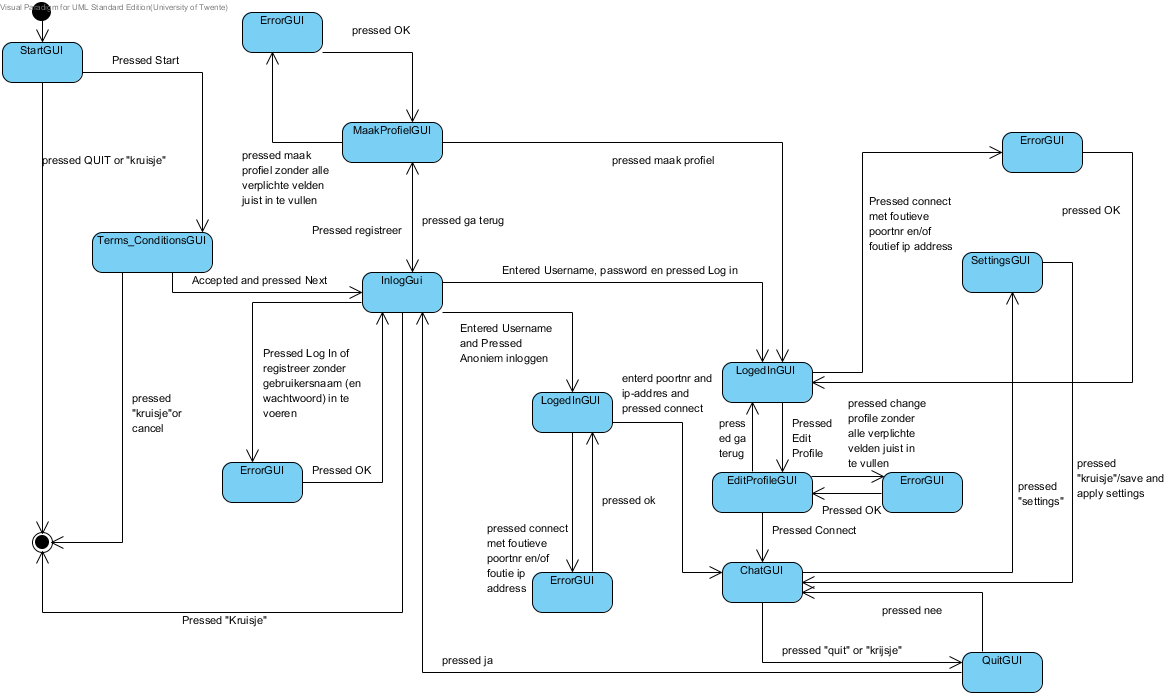
\includegraphics[width =230mm]{State_chart_GUI}
\caption{De state magine diagram van de graphic user interface}
\label{figure017}
\end{center}
\end{figure}
\end{landscape}
\newpage
\pagebreak[4]
\global\pdfpageattr\expandafter{\the\pdfpageattr/Rotate 0}

\section{Grafisch Ontwerp}
\label{aangegeven}
Voor het grafisch ontwerp is er gekozen om meerdere user interfaces te maken met elk hun eigen thema(in section 5.1 Schetsen wordt hier dieper op in gegaan). Voor een user interface is het van belang dat er meerdere windows gemaakt worden, er mag niet vanuit worden gegaan dat de gebruikers van de chatapplicatie het begrijpen en daarom moet de user interface hen bij de hand nemen.  Er is gekozen om losstaande Graphical User Interfaces te ontwerpen met allebei meerdere windows. De ChatGUI waar op pagina~\pageref{ChatGUI} verder op in wordt gegaan bevat drie aparte windows en de ConnectGUI waar op pagina~\pageref{ConnectGUI} verder op in wordt gegaan bevat twee aparte windows. De ConnectGUI zal gebruikt worden voor de gebruikers om hun gegevens op te geven en stelt ze in staat om een profiel aan te maken en te verbinden met de andere chatters. De ConnectGUI zal de gebruikers overdragen aan de ChatGUI die de rest van de sessie afhandelt totdat er afgesloten wordt.

\subsection{Schetsen}
De eerste versie van de ChatGUI lijkt nagenoeg op de uiteindelijk gekozen versie van de ChatGUI. Er ontbreken echter wat features in de eerste versie, zoals profiel ondersteuning, een instellingen knop en een  logout knop. Deze zijn er in de brainstorm bijgekomen in de uiteindelijke versie dat uit de doeken wordt gedaan op pagina~\pageref{Chat Window}. \\
De eerste versie van de ChatGUI zoals te zien is in figuur~\ref{figure001} is een statisch ontwerp dat in eerste instantie alle requirements voor een ChatGUI bevat.
%Hier ChGDv1%
\begin{figure}[ht]
\begin{center}
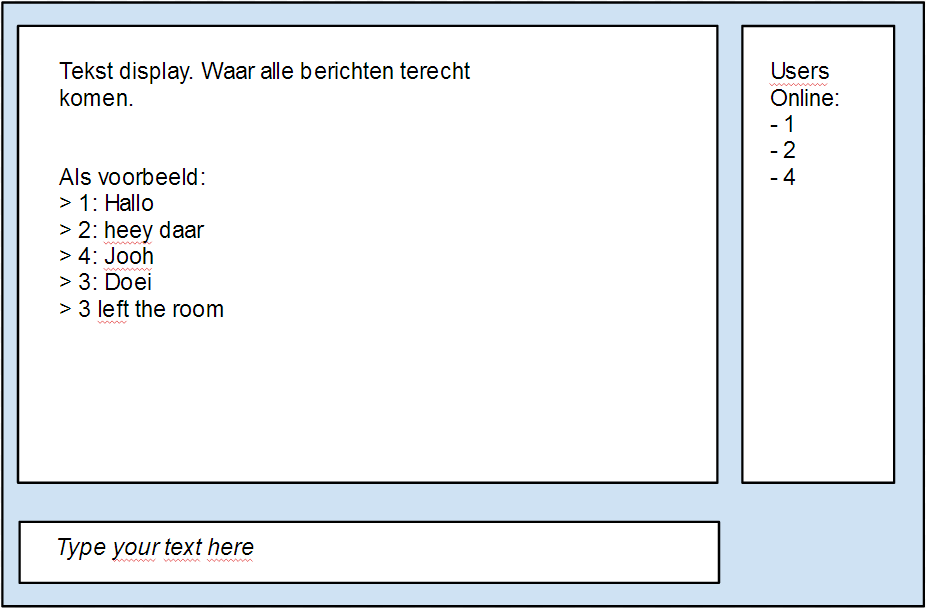
\includegraphics[width =90mm]{ChGDv1}
\caption{De eerste versie van de ChatGUI}
\label{figure001}
\end{center}
\end{figure}
\\

\noindent De tweede versie van de ChatGUI is in tegenstelling van de eerste versie en van de uiteindelijke versie niet strak maar legt de nadruk op rondingen en heeft een speels ontwerp zoals te zien is in figuur~\ref{figure002}.
%Hier ChGDv2%
\begin{figure}[ht]
\begin{center}
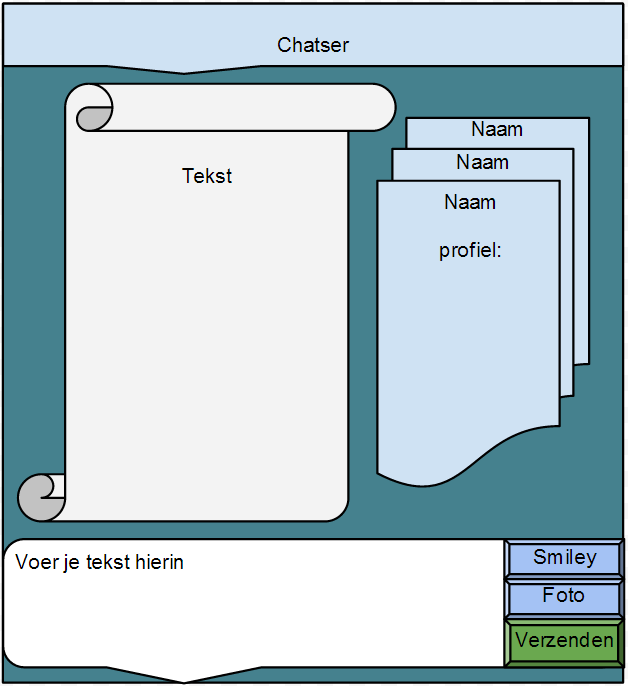
\includegraphics[width = 90mm]{ChGDv2}
\caption{De tweede versie van de ChatGUI}
\label{figure002}
\end{center}
\end{figure}
\\

\noindent De derde versie van de ChatGUI is ook onze uiteindelijk gekozen ontwerp voor de chat window, logout window en de settings window. Er zal op pagina~\pageref{ChatGUI} verder ingegaan worden op de redenen voor het kiezen van dit ontwerp. Het ontwerp dat we geschetst hebben ziet is te vinden in figuur~\ref{figure003} op pagina~\pageref{figure003}.
\label{ChGv3Chat}
%Hier ChGv3%
\begin{figure}[ht]
\begin{center}
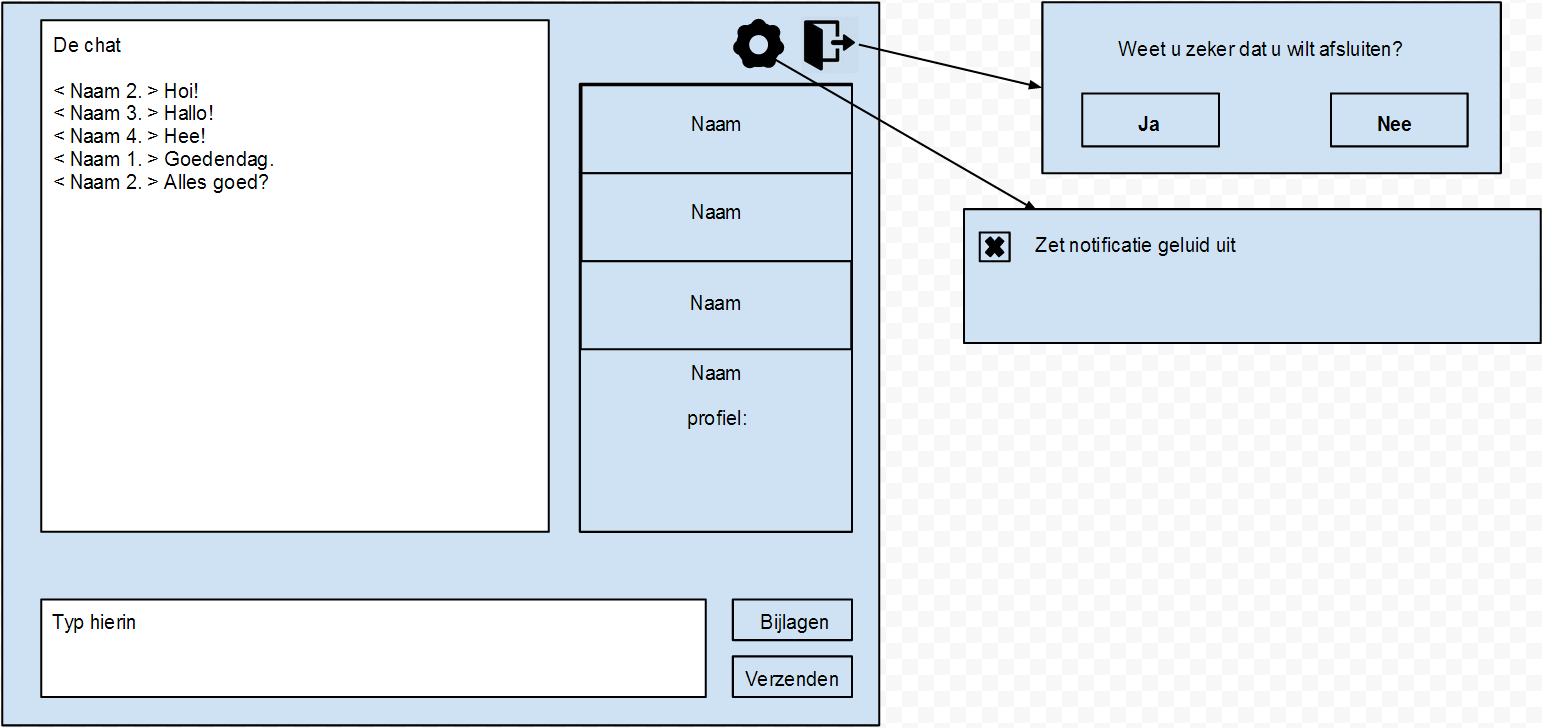
\includegraphics[width = 150mm]{ChGDv3}
\caption{De derde versie van de ChatGUI}
\label{figure003}
\end{center}
\end{figure}
\\

\noindent De eerste ConnectGUI is heel basaal en bevat enkel een tekstveld en een "connect"-knop en ondersteunt om die reden weinig functionaliteiten zoals te zien is in figuur~\ref{figure004} op pagina~\pageref{figure004}..
%Hier CGv1%
\begin{figure}[ht]
\begin{center}
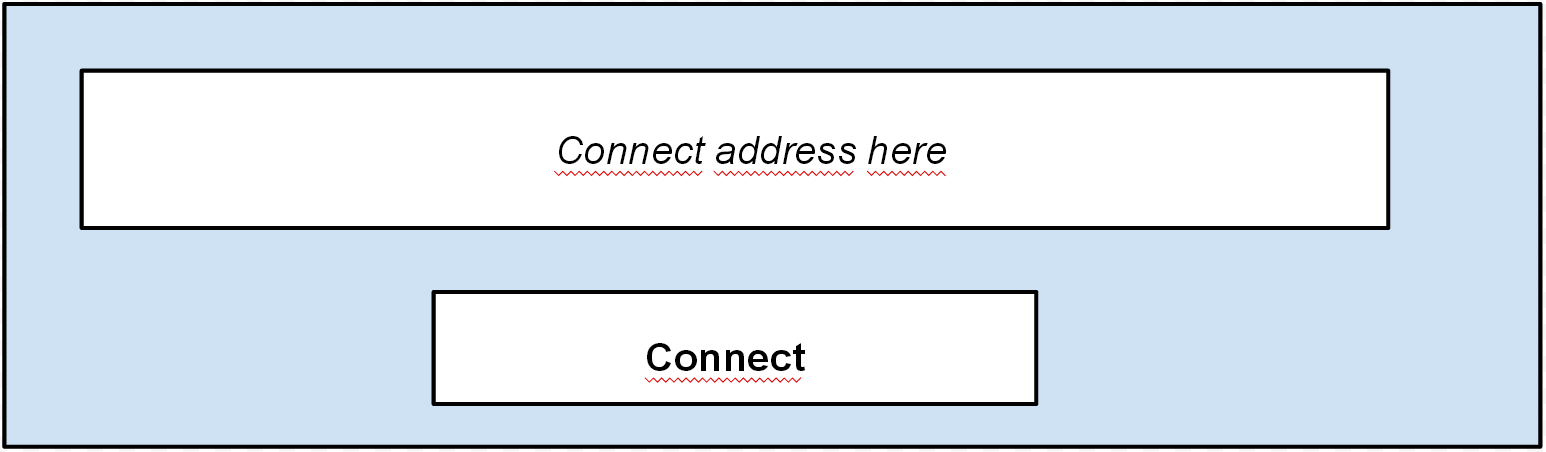
\includegraphics[width = 60mm]{CGDv1}
\caption{De eerste versie van de ConnectGUI}
\label{figure004}
\end{center}
\end{figure}
\\

\noindent De tweede ConnectGUI voegt \'e\'en functionaliteit toe aan het eerste ontwerp en dat is de functie om je alias op te geven en het ontwerp is net iets anders gestructureerd zoals te zien is in figuur~\ref{figure005} op pagina~\pageref{figure005}.
%Hier CGv2%
\begin{figure}[ht]
\begin{center}
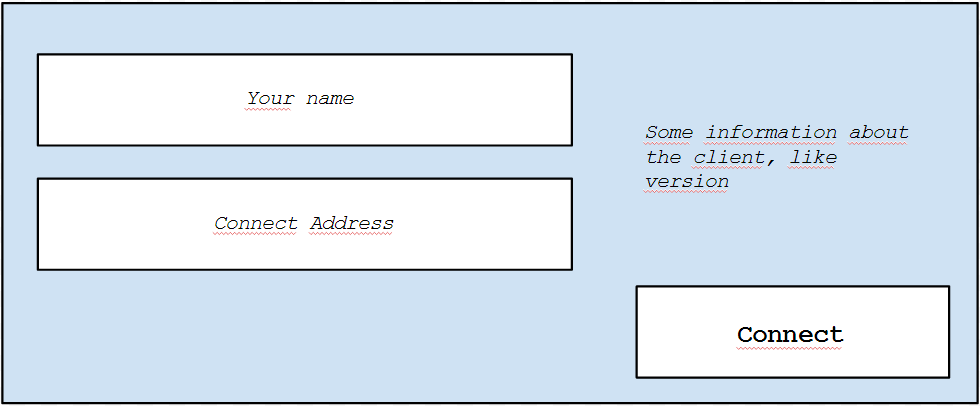
\includegraphics[width = 60mm]{CGDv2}
\caption{De tweede versie van de ConnectGUI}
\label{figure005}
\end{center}
\end{figure}
\\

\noindent De derde ConnectGUI voegt op zijn beurt weer een functionaliteit toe aan het tweede ontwerp en dat is een "Maak profiel aan" knop. Deze knop navigeert naar een ander window, de create profile window waar op pagina~\pageref{CPW} verder op in wordt gegaan. In figuur~\ref{figure006} op pagina~\pageref{figure006} kunnen de requirements worden afgelezen.
%Hier CGv3%
\begin{figure}[ht]
\begin{center}
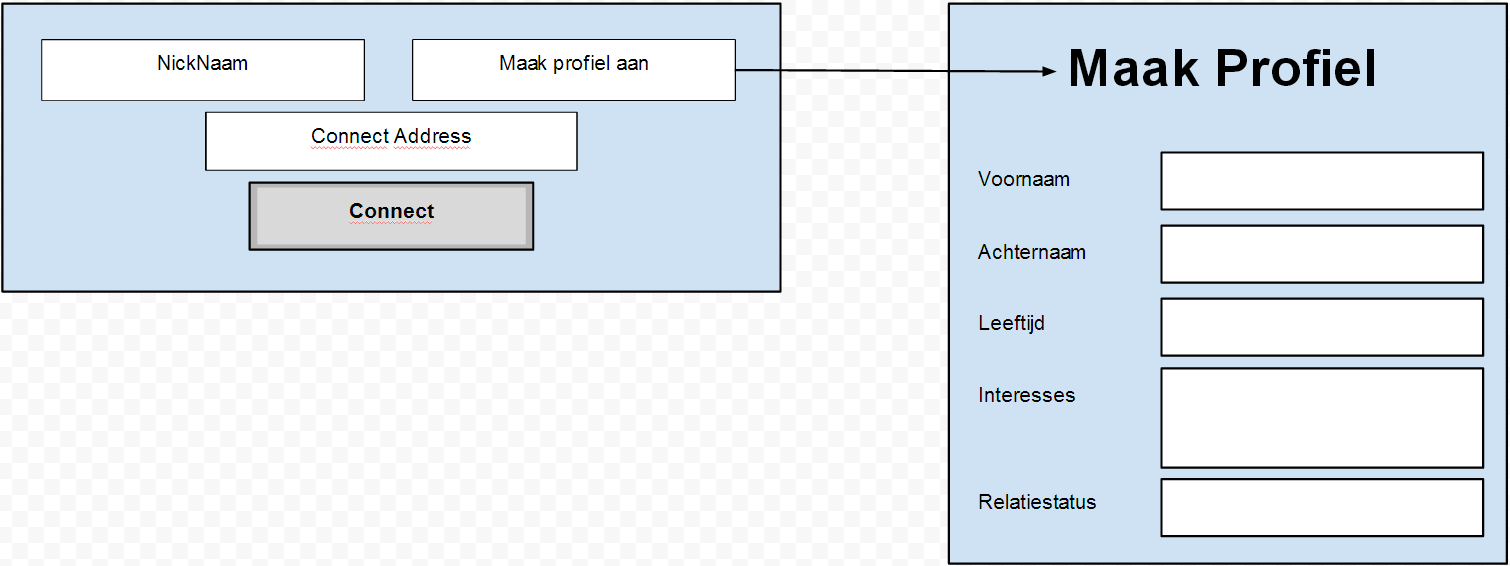
\includegraphics[width = 110mm]{CGDv3}
\caption{De derde versie van de ConnectGUI}
\label{figure006}
\end{center}
\end{figure}

\subsection{ChatGUI versie 3(ChGv3)}
\label{ChatGUI}
Er is gekozen na het maken van de schetsen om voor de laatste versie van de ChatGUI te kiezen. Deze versie is de derde gemaakte versie en is om die reden omgedoopt tot ChGv3. \\

\noindent Met het implementeren van ChGv3 als de ChatGUI is het de bedoeling dat het gebruiken van de applicatie niet lang aan het ontwerp te moeten wennen als deze gebruikt wordt naast andere applicaties. Om dit te bereiken zijn er een drietal peilers waar het ontwerp op is gebaseerd:
\begin{itemize}
\item{Strak Ontwerp}
\item{Schaalbaarheid}
\item{Overzicht}
\end{itemize}
Met deze drie peilers is het doel om een gebruiksvriendelijke applicatie te maken voor iedereen om te gebruiken. In de volgende subsections zullen deze drie peilers terugkomen.

\subsection*{Chat Window}
\label{Chat Window}
Zoals te zien is op pagina~\pageref{ChGv3Chat} is het ontwerp van de chat window strak, schaalbaar en overzichtelijk. De drie peilers komen respectievelijk terug in de rechthoekige vormen, schaalbare onderdelen en de layout. Er zijn twee chat window versies dat gebruikt worden. Een versie voor twee gebruikers en een versie voor 4 gebruikers.\\

\noindent De structuur van de chatwindow is hetzelfde opgebouwd als alle andere bekende (mobiele) chatapplicaties. Wij wilden echter de tekstveld voor de chat benadrukken en om die reden is deze zeer groot ten opzichten van alle andere onderdelen in de window en als gevolg van deze keuze zijn de namen van de andere mensen waarmee gechat word naar de zijkant verplaatst. Deze namen zijn knoppen die met een klik het profiel tekstveld onder de namen naar het profiel van diegene wiens naam is aangeklikt verandert. \\

\noindent Rechtsboven aan zijn er twee knoppen, de settings knop en een logout knop. Deze twee knoppen navigeren naar de windows die op pagina~\pageref{LWSW} uitgelegd worden.

\subsection*{Settings Window en Logout Window}
\label{LWSW}
De settings window heeft \'e\'en optie dat aangevinkt kan worden door een checkbox en dat is de optie of de notificatiegeluid aan of uit moet. Bovendien word de software versie van de applicatie aangegeven.
\\

\noindent De logout window bevat de vraag of de gebruiker echt uit de chat wil stappen en de twee knoppen Ja en Nee. Als er op Nee geklikt word dan zal de logout window gesloten worden. Als er voor Ja gekozen wordt dan zal zowel de logout window als de chat window gesloten worden en de gebruiker wordt genavigeerd naar de connect window van de ConnectGUI wat op pagina~\pageref{connectie}  word uitgelegd.

\subsection{ConnectGUI versie 3(CGv3)}
\label{ConnectGUI}
De connectGUI bestaat zoals al aangegeven op pagina~\pageref{aangegeven} uit twee verschillende windows, de connect window en de create profile window. Deze twee windows zijn de portalen naar de chat window. De gebruiker hoeft geen profiel aan te maken als het 'anoniem' wil chatten met anderen. Als de gebruiker een profiel wil hebben dan is dat mogelijk door op de "Maak profiel aan" knop te klikken.

\subsection*{Connect Window}
\label{connectie}
De connect window heeft twee tekstvelden en twee knoppen. Deze twee tekstvelden zijn voor het invullen van je alias en de ander is voor je adres dat een IPv4 adres is waar de 24 bytes vaststaan en de laaste vier bytes staat voor de devicesnumber dat de gebruiker heeft. Dit kan dus 1, 2, 3 of 4 zijn. De twee knoppen zijn om een profiel aan te maken en om te verbinden. De "maak profiel aan" knop navigeert naar de create profile window en de "connect" knop navigeert naar de chat window.

\subsection*{Create Profile Window}
\label{CPW}
De create profile window heeft vijf tekstvelden die ingevuld kunnen worden. De velden voor de voornaam, achternaam en leeftijd zijn verplicht en deze verplichte velden worden aangegeven met een(*). De overige twee velden, interesses en relatie status zijn niet verplicht. Het invullen van de verplichte velden zijn alleen verplicht als er een profiel aangemaakt word. Dus als de gebruiker geen profiel aan wil maken dan zijn deze velden uiteraard niet verplicht om in te vullen. 
\newpage

\section{Resultaten}
In deze section zullen de resultaten van het netwerk ontwerp en van het software ontwerp besproken worden. Voor het netwerk ontwerp gedeelte zal het afhandelen van de backend gedeelte centraal komen te staan en voor het grafische ontwerp zal het belangrijk zijn om naar de user interfaces te kijken die uiteindelijk gemaakt zijn na de gemaakte schetsen. 

\subsection{Netwerk Ontwerp}
Het netwerk dat ge\"implementeerd is kan berichten versturen tussen twee gebruikers en tussen vier gebruikers. Tijdens het mogelijk maken van het versturen van bestanden met verschillende extensies was het nodig om via invoer de bestandsnaam op te geven om het te kunnen versturen naar de anderen. De anderen moeten dan naar de map gaan waar het in zou moeten komen te staan en daar zal het bestand gevonden kunnen worden. In de eindversie kunnen de bestanden aangeklikt worden en worden deze geopend.

\subsection{Grafisch Ontwerp}
De gemaakte chat windows lijken veel op de schets dat gemaakt is. Er was geen schets gemaakt voor de twee gebruikers variant maar het enige verschil is dat voor de twee gebruikers versie dat de knoppen met namen er niet op staan. De twee versies zijn uiteindelijk eruit komen te zien zoals in figuur~\ref{figure007} en figuur~\ref{figure008} te zien is.
%Hier de chat windows%
\begin{figure}[ht]
\begin{center}
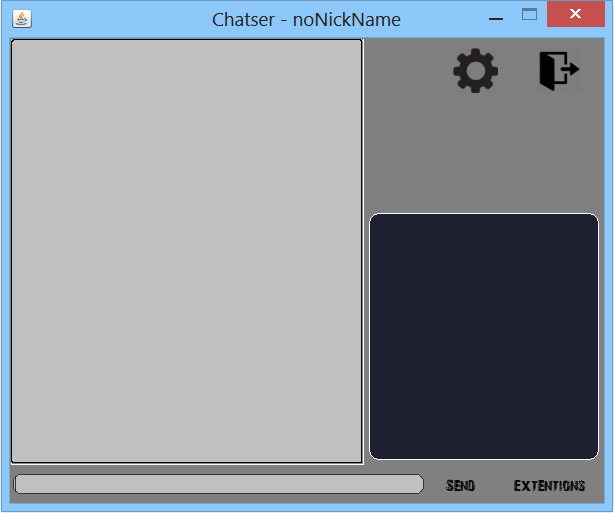
\includegraphics[width = 60mm]{chatser2}
\caption{De uiteindelijke versie van de ChatGUI voor 2 personen}
\label{figure007}
\end{center}
\end{figure}

\begin{figure}[ht]
\begin{center}
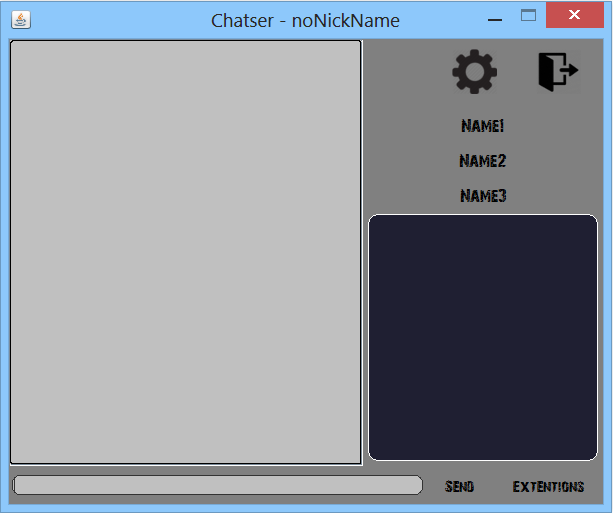
\includegraphics[width = 60mm]{chatser}
\caption{De uiteindelijke versie van de ChatGUI voor 4 personen}
\label{figure008}
\end{center}
\end{figure}
\noindent De settings window heeft tijdens de ontwikkelfase de software versie gekregen, dit stond in eerste instantie niet in het ontwerp, maar het was een mooie toevoeging. Deze settings window is te vinden in figuur~\ref{figure009}.
%Hier de settings window%
\begin{figure}[ht]
\begin{center}
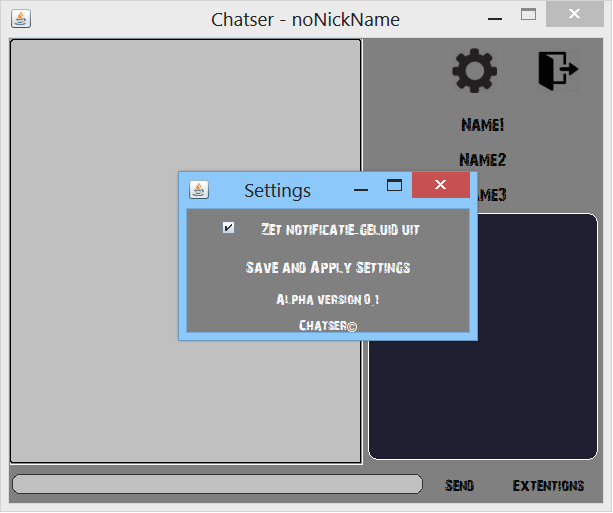
\includegraphics[width = 60mm]{chatsersettingsaan}
\caption{De uiteindelijke versie van de SettingGUI}
\label{figure009}
\end{center}
\end{figure}
\\

\noindent De logout window is na implementatie hetzelfde als de schets dat gemaakt is zoals in figuur~\ref{figure010} te zien is op de volgende pagina, dit omdat het een eenvoudig ontwerp had.
%Hier de logout window%
\begin{figure}[ht]
\begin{center}
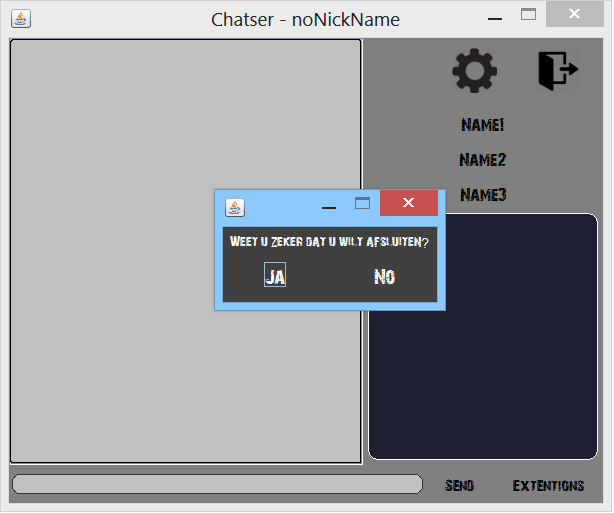
\includegraphics[width = 60mm]{chatserafsluiten}
\caption{De uiteindelijke versie van de logout window}
\label{figure010}
\end{center}
\end{figure}
\\
\newpage
\noindent De connect window heeft tijdens de ontwikkelfase een keuze blok erbij gekregen waarin kan worden met hoeveel gebruikers er gechat wil worden, als gevolg hiervan wordt de gebruiker altijd naar de goede chat window genavigeerd zoals in figuur~\ref{figure011} te zien is.
%Hier de connect window%
\begin{figure}[ht]
\begin{center}
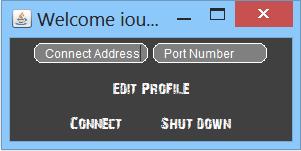
\includegraphics[width = 60mm]{connection_met_profiel}
\caption{De uiteindelijke versie van de connect window}
\label{figure011}
\end{center}
\end{figure}
\\

\noindent De create profile window heeft een paar wijzigingen ten opzichte van het ontwerp. De tekstvelden zijn even groot en dus ook de interesses veld is van gelijke grootte als de andere velden. Ook is er een paneelnaam toegevoegd zodat de window er wat gelikter uit kwam te zien. Ook Zijn er knoppen toegevoegd aan de onderkant om terug te navigeren naar de connect window. De ene knop slaat de gegevens op en de ander niet, mocht de gebruiker toch geen profiel willen. Dit is de vinden in figuur~\ref{figure012} op pagina~\pageref{figure012}.
%Hier de create profile window%
\begin{figure}[ht]
\begin{center}
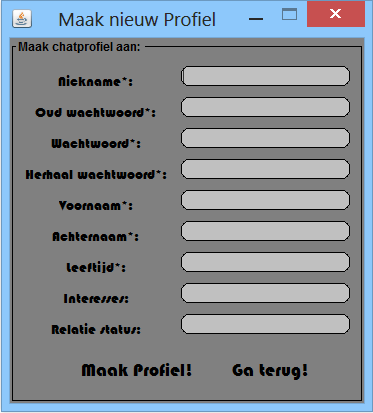
\includegraphics[width = 60mm]{MaakProfielGUI}
\caption{De uiteindelijke versie van de create profile window}
\label{figure012}
\end{center}
\end{figure}
\\
\newpage
\noindent Er zijn wat extra windows bijgekomen. Dit zijn de startscherm, de terms and conditions scherm,  een connect account scherm en een inlog scherm. Ook zijn er een directory scherm een emoticon scherm en een keuze scherm erbij gekomen. Bovendien is er een veranderbare error! scherm toegevoegd.
\\

\noindent In figuur~\ref{figure013} op pagina~\pageref{figure013} worden ze emoticons weergegeven die zijn toegevoegd aan de applicatie om de gebruiker ondersteuning van emoticons te bieden die een uitdrukking van de gebruiker kan versterken.
%overige schermen%
\begin{figure}[ht]
\begin{center}
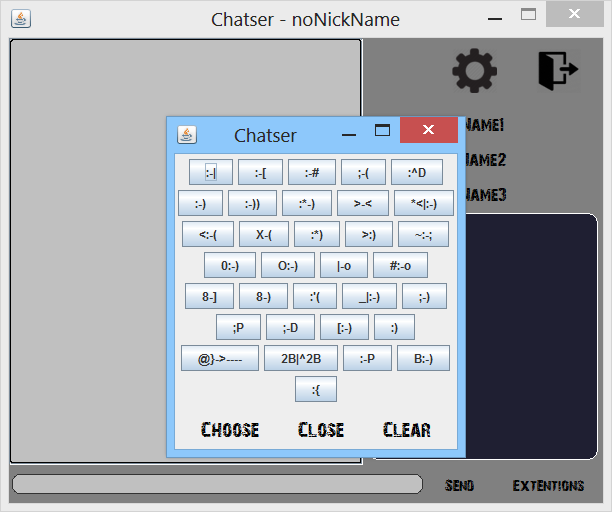
\includegraphics[width = 90mm]{chatser_emoticons}
\caption{De uiteindelijke versie van de emoticon window}
\label{figure013}
\end{center}
\end{figure}
\\

\noindent In figuur~\ref{figure014} op pagina~\pageref{figure014} worden de extensies weergegeven. Deze extensies moeten het mogelijk maken om files te sturen voor de Chatser-applicatie\small\textcopyright.
\begin{figure}[!h]
\begin{center}
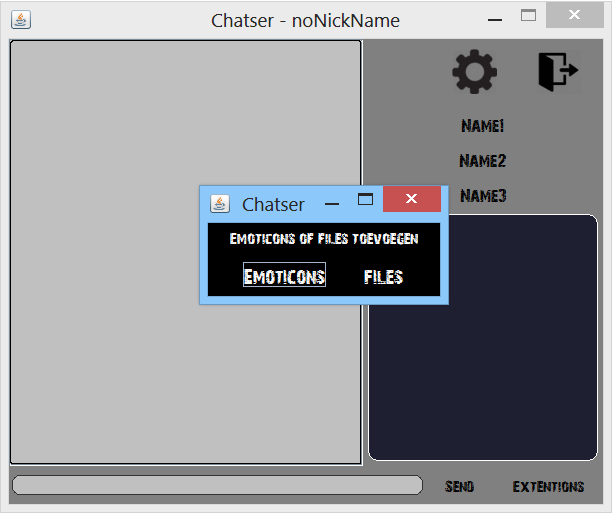
\includegraphics[width = 90mm]{chatser_extentions}
\caption{De uiteindelijke versie van de extentions window}
\label{figure014}
\end{center}
\end{figure}
\\

\noindent In figuur~\ref{figure015} op pagina~\pageref{figure015} wordt de StartGUI weergegeven. Dit scherm is het eerste scherm dat gebruiker te zien krijgt als de applicatie opgestart wordt.
\begin{figure}[!h]
\begin{center}
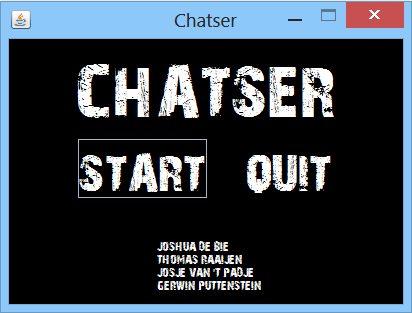
\includegraphics[width = 90mm]{StartGUI}
\caption{De uiteindelijke versie van de start window}
\label{figure015}
\end{center}
\end{figure}
\\

\noindent In figuur~\ref{figure016} op pagina~\pageref{figure016} wordt het terms and conditions scherm weergegeven, dit is het tweede scherm dat de gebruiker te zien krijgt. De gebruiker moet eerst instemmen met de voorwaarden om verder te kunnen naar het inlogscherm. \newpage

\begin{figure}[!h]
\begin{center}
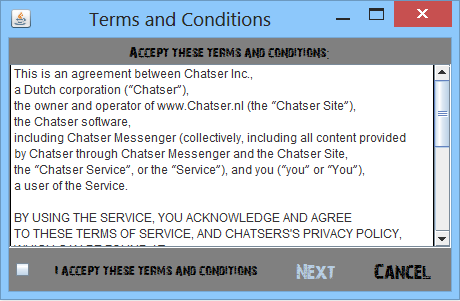
\includegraphics[width = 90mm]{Terms_Conditions1}
\caption{De uiteindelijke versie van terms and conditions window}
\label{figure016}
\end{center}
\end{figure}

\newpage

\section{Conclusie}
Met het resultaat zijn het netwerk ontwerp en het grafische ontwerp bij elkaar gekomen.  het ad-hoc netwerk samen met de multi-hop en de chatGUI zijn het hart van de applicatie.  Ook is de applicatie goed beveiligd door de berichten goed te versleutelen en moeten de gebruikers die als henzelf willen chatten door een profiel zich kunnen verifi\"eren door middel van een wachtwoord die gecheckt word door het te hashen. Er is maar een applicatie dit het doet zoal geen ander het doet en dat is de Chatser-applicatie\small\textcopyright.

\newpage

\section{Nawoord}
Wij als gehele groep hebben dit project als zeer plezant ervaren. Tijdens het project hebben wij zoals op pagina~\pageref{taken} de taken verdeelt. Hierdoor was het team in staat om elk teamlid een aparte taak te geven om effectief te werk te kunnen gaan. Het resultaat van het project is zoals het voor ogen was binnen de groep. Een goed werkend systeem waarmee alle bestandsformaten kunnen  worden verstuurd onder een mooie voorkant, wat de GUI moet zijn. De hoop is dat de GUI voor een goede gebruikerservaring gaat zorgen voor een geavanceerde chatapplicatie. Het achterliggende idee is dat er geen andere applicatie zo'n goede gebruikerservaring zal bieden zoals de Chatser-applicatie\small.\textcopyright!


\end{document}
